\label{703}
Gehen Sie wie folgt vor, um das Integral
\[
I=\int_{-\infty}^{\infty} \frac1{x^2 + 1}\,dx
\]
zu berechnen.
\begin{teilaufgaben}
\item Schreiben Sie den Integranden in den Form
\begin{equation}
f(z)=A\biggl(\frac{1}{z-z_1} - \frac{1}{z-z_2}\biggr),
\label{702:fz}
\end{equation}
wobei die Zahlen $a$ und $b$ komplex sein d"urfen (Partialbruchzerlegung).
\item
Verwenden Sie die Cauchy-Integralformel um das Integral
\[
I_R
=
\oint_{\gamma_R}f(z)\,dz,
\]
zu berechnen,
wobei $\gamma_R$ der Weg ist, der sich aus den zwei Teilst"ucken
\[
\begin{aligned}
\gamma_1(t)&=t&&\text{f"ur $t\in[-R,R]$}\\
\gamma_2(t)&=Re^{it}&&\text{f"ur $t\in[0,\pi]$}
\end{aligned}
\]
zusammensetzt (Abbildung~\ref{703:path}).
\begin{figure}
\centering
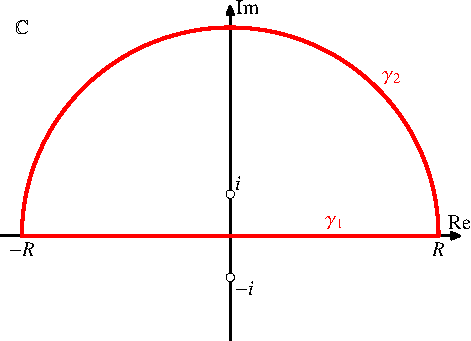
\includegraphics{../skript/uebungsaufgaben/path-1.pdf}
\caption{Pfad zur Berechnung des Integrals in Aufgabe\ref{703}
\label{703:path}}
\end{figure}
\item 
Versichern Sie sich, dass beim Grenz"ubergang $R\to\infty$ das Integral
entlang $\gamma_1$ zum gesuchten Integral $I$ wird.
\item
"Uberlegen Sie sich den Grenzwert des Integrals entlang des Teilst"ucks
$\gamma_2$ f"ur $R\to\infty$.
\item
Leiten Sie daraus den Wert von $I$ ab.
\end{teilaufgaben}

\begin{loesung}
\begin{teilaufgaben}
\item
Bringt man den Ansatz auf einen Nenner, erh"alt man
\[
\frac1Af(z)
=
\frac{(z-z_2)-(z-z_1)}{(z-z_1)(z-z_2)}
=
\frac{(z-z_2)-(z-z_1)}{z^2-(z_1+z_2)z-z_1z_2}
=
\frac{-z_2+z_1}{z^2-(z_1+z_2)z+z_1z_2}
\]
Da im Nenner kein linearer Term in $z$ vorkommen darf, folgt
$z_1+z_2=0$ oder $z_1=-z_2$.
Der konstante Term muss $1$ werden, also $z_1z_2=-z_1^2=1$,
somit muss $z_1=i$ und $z_2=-i$ (oder umgekehrt) sein.
Mit diesen Werten wird $f(z)$ zu
\[
f(z)=A\frac{2i}{z^2+1},
\]
um den Integranden zu bekommen, muss man also $A=\frac1{2i}$ verwenden.
\item
Setzt man die in a) gefundene Form f"ur $f(z)$ in das Integral ein, erh"alt
man
\[
\oint_\gamma f(z)\,dz
=
\frac1{2i}
\oint_\gamma
\frac{1}{z-i}-\frac{1}{z+i}\,dz
=
\frac1{2i} \oint_\gamma \frac{1}{z-i}\,dz
-
\frac1{2i}
\underbrace{\oint_\gamma \frac{1}{z+i}\,dz}_{\textstyle=0}
\]
Der erste Term sieht aus wie die Cauchy-Integral-Formel f"ur die konstante
Funktion $1$:
\[
1=\frac1{2\pi i}\int_\gamma \frac{1}{z-a}\,dz,
\]
wir schliessen daher, dass dieser Term den Wert $\pi$ haben muss.
Somit gilt
\[
\oint_\gamma f(z)\,dz
=
\pi.
\]
\item
Das $\gamma_1$-Integral ist
\begin{align*}
\int_{\gamma_1} f(z)\,dz &= \int_{-R}^{R} \frac1{t^2+1}\,dt
\end{align*}
f"ur $R\to\infty$ also genau das gesuchte Integral.
\item
Das Integral entlang $\gamma_2$ ist
\begin{align*}
\biggl|\int_{\gamma_2} f(z)\,dz\biggr|
&
\le
\int_0^\pi \frac1{|z^2+1|} |iRe^{it}|\,dt
<
\int_0^\pi \frac1{R^2} R\,dt
=\frac{\pi}{R},
\end{align*}
geht also f"ur $R\to\infty$ gegen 0.
\item
F"ur $R\to\infty$ bekommen wir also
\begin{align*}
\pi
&=
\lim_{R\to\infty}\oint_{\gamma} f(z)\,dz
=
\lim_{R\to\infty}\int_{\gamma_1} f(z)\,dz
+
\lim_{R\to\infty}\int_{\gamma_2} f(z)\,dz
\\
&=
\int_{-\infty}^{\infty} \frac1{t^2+1}\,dt + 0 = I.
\end{align*}
Wir lesen ab: $I=\pi$.
\qedhere
\end{teilaufgaben}
\end{loesung}


